\documentclass[a1paper,fontsize=24.88pt,twoside=false,english,DIV=calc,NET]{scrartcl}

\usepackage{wrapfig}

\usepackage{svg}
% size should not be changed unless explicitely instructed otherwise
\usepackage{geometry}
\geometry{paperwidth=600mm, paperheight=800mm, left=35mm,right=35mm, top=35mm, bottom=35mm} % I8 framesize

% sizes

\newcommand{\headervspace}{26mm} % A1/I8
\newcommand{\logoheight}{26mm} % A1/I8

\usepackage{posterstyle}

% ===============================================================
% Font settings
% ===============================================================
\usepackage{helvet}
\renewcommand{\familydefault}{\sfdefault}
\fontfamily{phv}\selectfont
\renewcommand{\rmdefault}{lhv}
\renewcommand{\seriesdefault}{m}
\renewcommand{\shapedefault}{n}
\DeclareSymbolFont{operators}{OT1}{cmbr}{m}{n}
\DeclareSymbolFont{letters}{OML}{cmbrm}{m}{it}
\DeclareSymbolFont{symbols}{OMS}{cmbrs}{m}{n}
% ===============================================================

% Type and title of your work, please adhere to the following format:
% {Bachelor' Thesis | Master's Thesis | Interdisciplinary Project | Guided Research}: title,
\def\titletext{Bachelor's Thesis: Performance-Analysis of VPP}

% Adapt font size to fit in a single line
\newcommand{\titlefontsize}{\fontsize{36}{40}\selectfont} % A1/I8

% Fill in the name of the persons
\def\presenter{Peter Okelmann}
\def\advisor{Paul Emmerich, Dominik Scholz}
\def\supervisor{Prof. Dr.-Ing. Georg Carle}

\begin{document}

\TUMheader[TUMDarkerBlue]{\logoheight}

\begin{wrapfigure}[10]{r}{3in}
\centering

\includegraphics[width=2in]{pics/logo_fdio.png}
\end{wrapfigure}

\vspace{\headervspace}


{{\titlefontsize \titletext \\}

\vspace{-1.5ex}
{{\fontsize{28}{32}\strut\selectfont Intermediate Talk\\}

\vspace{.8\headervspace}

\ssingletextbox{\footnotesize \textcolor{TUMDarkerBlue}{ {\textit{Presenter:} \presenter --- \textit{Advisors:} \advisor --- \textit{Supervisor:} \supervisor }  \hspace*{\fill} }}
%\ssingletextbox{\footnotesize \textcolor{TUMDarkerBlue}{{} \hspace*{\fill}}}

\doubletextbox{35ex}{VPP: a fast software router}{
	\footnotesize
	VPP (Vector Packet Processing) is a user-space software router. This approach combines many advantages:
	\begin{itemize}
		\item deployable to usual architechtures
		\item fast user-space network interface drivers
		\item can run in virtualized containers
	\end{itemize}
	\vspace{2ex}

	"It is the open source version of Cisco's Vector Packet Processing (VPP) technology."\cite{vppwiki:whatis} 
	Now it is beeing developed by FD.io ("The Fast Data Project") which belongs to the Linux Foundation. 

	Feature Highlights:
	\begin{itemize}
		\item vecorized processing of packets in badges
		\item utilizes high-speed dpdk drivers
		\item modular and extendable packet-processing graph
		\item cpu-scalability
	\end{itemize}
}{Testing Methodology}{
	\footnotesize
	MoonGen\cite{moongen-imc2015} is scripted to generate testing load according to the following testing parameters:
	\begin{itemize}
		\item packet rate
		\item packet size
		\item traffic type (generic Ethernet, UDP)
		\item traffic pattern (inter packet gaps)
	\end{itemize}
	\footnotesize
	Gathered testing results:
	\begin{itemize}
		\item latency histogram
		\item throughput
		\item linux perf stats (cache misses...)
		\item linux perf record (cpu-time spent per symbol)
		\item internal vpp state information
	\end{itemize}
	\footnotesize
	For tests to return meaningful results, the optimum of throughput to latency is beeing found by a script. This packet rate is then used for further tests. Otherwise the results are inaccurate, because of utilization of the packet buffer.  
	\footnotesize
	VPP properties to test:
	\begin{itemize}
		\item raw forwarding throughput
		\item latency: cache and memory impact
		\item packet processing graphs utilizing multiple cpu cores
		\item testing specific processing nodes / router features
	\end{itemize}
}

\vfill

\doubletextbox{39ex}{Measurement setup}{
	Background
	\footnotesize
	\begin{itemize}
		\item Important background for this work
		\item may be some things about related work or important libraries/frameworks used
	\end{itemize}
	\footnotesize
	Measurment Setup:
	\begin{itemize}
		\item How does your setup look like (maybe a figure)?
		\item What are the relevant questions you try to answer with your measurement?
		\item What do you measure?
		\item How do you measure?
	\end{itemize}
}{Benchmarking Setup}{
	\footnotesize
	\begin{center}
		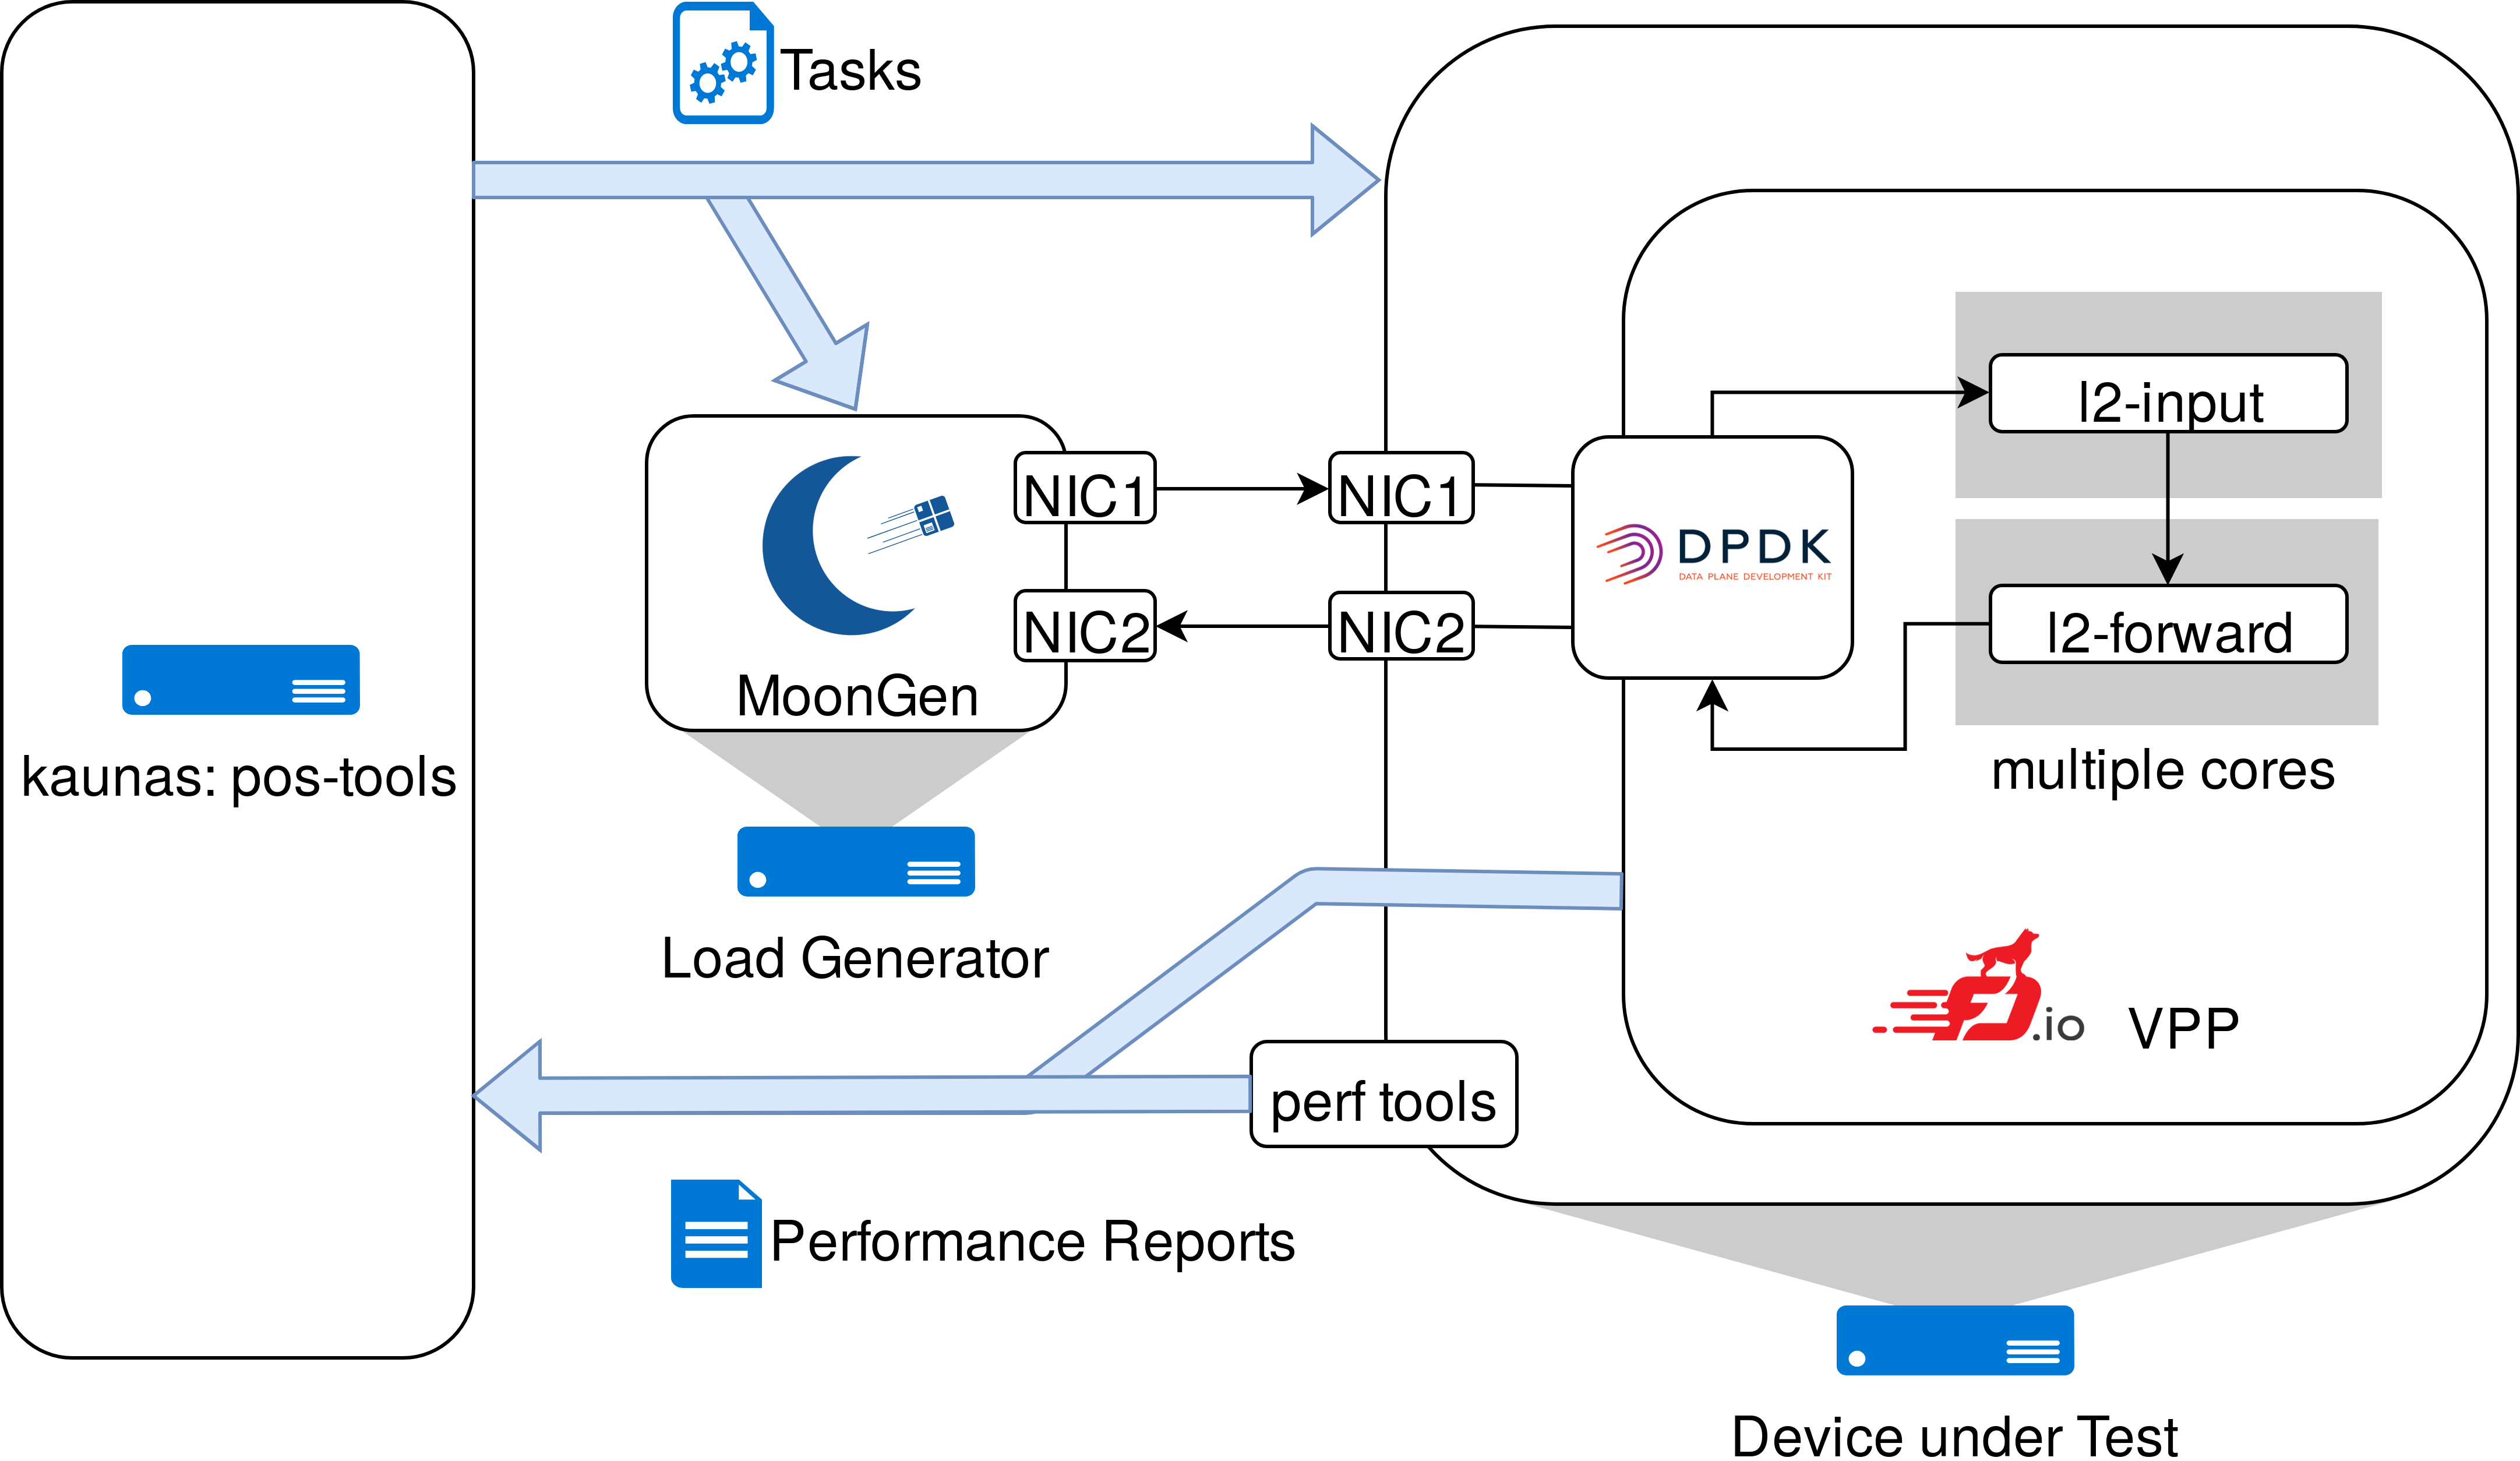
\includegraphics[width=24cm]{pics/topology2.png}
		% \includesvg[width=14cm]{../../../pics/topology}
	\end{center}
}

\vfill

\doubletextbox{28ex}{l2 Throughput}{

	\footnotesize
	The following results are produced by sending non-ip ethernet packets to a single destination. VPP ran on an Intel E5-2640 @ 2.0GHz (cesis) with 10G networking results in the following numbers:

	\vspace{5ex}
	\centering
	\begin{tabular}[]{ l r r r}
		\footnotesize
		VPP config & max Mpps & stable Mpps & Relative \\
		\midrule
		packet gen speed & 14.86 & 14.86 & 100\% \\
		l2 xconnect & 10.4 & 10.1 & 68\% \\
		l2 bridge: no features & 9.35 & 9.2 & 62\% \\
		l2 bridge: mac-age & 8.62 & 8.6 & 58\% \\
		l2 bridge: mac-learn & 8.51 & 8.3 & 56\% \\
		l2 bridge: mac-learn, mac-age & 8.50 & 8.3 & 56\%
	\end{tabular}


	\vspace{5ex}
	\centering
	\begin{tabular}[]{ l r r r}
		\footnotesize
		Router                                      & Mpps & Relative \\
		\midrule
		MoonRoute                                   & 14.6 & 100\%    \\
		FastClick (DPDK 2.2)~\cite{moongen-imc2015} & 10.4 & 72\%     \\
		Click (DPDK 2.2)~\cite{moongen-imc2015}     & 4.3  & 29\%     \\
		Linux 3.7                                   & 1.5  & 10\%
	\end{tabular}

}
{Planned Schedule}{
	\footnotesize
	Short time schedule for the upcoming weeks:

	\begin{itemize}
		\item Official start date: October 15, 2010
		\item Official end date: February 15, 2011
		\item Weeks left: 8
	\end{itemize}
	
	\textbf{Schedule}
	\begin{itemize}
		\item Week 1-4: Providing cookies for I8
		\item Week 5-6: Perform additional measurements
		\item Week 7: Writing thesis
		\item Week 8: \textbf{Several} corrections passes
		\item Week 9: Print and hand-in
	\end{itemize}
}

\vfill 

% This is the literature box.
% There the most relevant papers related to the presented work are listed.
\notitlesingletextbox{13ex}{
	\nocite{moongen-imc2015}
	\nocite{guenthergf}
	\nocite{braun2010comparing}
	\nocite{netgames}
	%\nocite{ancs}%

	\vspace{-1ex}  
	\scriptsize
	\begingroup
		\renewcommand{\section}[2]{}%
		\bibliography{lit}
		\bibliographystyle{abbrv}
	\endgroup
}

\vfill

\end{document}